\chapter{力、クォーク、そして最初のハドロン多重項}

\section{粒子、場、そして欠けた第三の辺}

波は場の配位であるから、本稿の議論においてこの二つの記述は密接に関係している。量子力学によれば、そのような波のエネルギーは離散的で不可分な単位で現れる。その単位が量子であり、場の量子を我々は粒子と呼ぶ。この関係を手にした上で、我々はすでに波動方程式、作用原理、そして粒子が担う広範な性質——エネルギー、運動量、スピン、ボソン--フェルミオンという区別——について論じてきた。フェルミオンは同一状態を占めることに抵抗し、ボソンは集まり一つの状態へ凝縮しうる。

量子ラグランジアンは相互作用をも記録する。場の積は粒子が出入りする頂点を表す。例えば場の四乗を含む項は四本の脚をもつ相互作用頂点を表す。このようにして作用原理は、起こりうる粒子過程の簡潔な目録となる。

次の課題は粒子に名前を与えることである---一つ一つではなく、いくつかの族として---そしてそれぞれに個性を与えること、すなわちその性質、その相互作用、通常の物理学における位置づけである。しかしその一覧を作る前に、概念的三角形の一辺がまだ欠けている。
\begin{itemize}
\item 粒子、
\item それらの粒子が量子であるような場、
\item 同じ量子を含む交換過程に伴う力。
\end{itemize}

\emph{素}という語は暫定的なままでなければならない。複合粒子ではなく素粒子であるためのもっともらしい定義はどれも、やがて微妙な事例に突き当たる。この問題には後に戻る。今は基本場が存在すると仮定し、その量子を素粒子と呼ぶことにしよう。電場が電気的な力を生み、重力場が重力を生むのなら、電子場もまた力に関与しなければならない。三角形が閉じるのは、力が場による記述だけでなく粒子による記述をもつ場合に限られる。

したがって我々は力の論理を二度導出する。まず古典的な場のエネルギーを用い、次に同じ相互作用が場を量子に分解したときどのように現れるかを問う。その橋が確かなものになって初めて、粒子の目録が始まる。

\section{古典電気力学における場のエネルギーからの力}

二つの電荷を空間に置く。それらの力を求める一つの方法は逆二乗則を引用することである。より多くを明かす方法は、電荷が空間に何をするかを問うことである。すなわち電荷は電場を作り、その場がエネルギーを蓄える。

各電荷をその場の空間的な形から分離しておくと便利である。
\begin{equation}
\mathbf E_i=q_i\widehat{\mathbf E}_i,
\end{equation}
もっとも、ハット記法を保つことに何も依存しない。両方の電荷が存在するとき、線形性により
\begin{equation}
\mathbf{E}=\mathbf{E}_1+\mathbf{E}_2.
\end{equation}
単位の選び方を別にすれば、静電場のエネルギーは次の形をとる。
\begin{equation}
U_{\text{field}}\propto\int d^3x\,\mathbf{E}^2.
\end{equation}
二つの場の和を代入すると
\begin{align}
U_{\text{field}}
&\propto\int d^3x\,(\mathbf{E}_1+\mathbf{E}_2)^2 \\
&\propto\int d^3x\,\bigl(\mathbf{E}_1^2+\mathbf{E}_2^2
  +2\mathbf{E}_1\!\cdot\!\mathbf{E}_2\bigr).
\end{align}

最初の二つの項は自己エネルギーである。どちらの電荷を動かしてもその場はそれとともに動き、対応する積分は変化しない。そのエネルギーは\(E=mc^2\)を通じて、孤立した荷電粒子の測定質量に寄与する。この自己エネルギーがどのように測定質量に組み込まれるかは、後の繰り込みという主題に属する。この位置に依存しないエネルギーのいずれも、二つの粒子の間の力には寄与しない。

交差項は異なる。それはどちらの粒子にも単独には属さず、両方の場が存在するときにのみ存在する。電荷を非常に遠く離すと、それらの無視できない場の領域はほとんど重ならない。電荷が近づくにつれて重なりが変化する。したがって配位に依存する相互作用エネルギーは次に比例する。
\begin{equation}
U_{\text{int}}(r)\propto q_1q_2\int d^3x\,
\widehat{\mathbf E}_1\!\cdot\!\widehat{\mathbf E}_2.
\end{equation}
\(r\)だけ離れた二つの点電荷に対して、この積分を評価するとおなじみの依存性が得られる。
\begin{equation}
U_{\text{int}}(r)\propto\frac{q_1q_2}{r}.
\end{equation}
動径方向の力はその負の勾配であり、
\begin{equation}
\mathbf F_{12}=-\boldsymbol\nabla_{\mathbf r}U_{\text{int}},
\qquad
|\mathbf F_{12}|\propto\frac{|q_1q_2|}{r^2}.
\end{equation}
\editorialnote{口頭の議論はポテンシャルで立ち止まることなく、交差項を逆二乗のクーロン力と同一視する。標準的な中間量\(U_{\mathrm{int}}\propto1/r\)をここで明示的に書いたのは、その勾配が述べられた\(1/r^2\)の力を与えるようにするためである。}

力の法則は、相対位置を知っている場のエネルギーの部分の導関数となった。遠く離れれば、二つの物体は実質的に独立である。それらを近づけると、それらの間の場が再配置され、その結果生じるエネルギーの変化が相互作用である。

しかし場が量子に分解されうるのなら、これで話が終わるはずがない。同じ力が粒子の言語による説明をもたなければならない。

\section{分子交換：二つの陽子と一つの電子}

電気力学に戻る前に、交換をより描きやすい系を考えよう。2個の陽子と1個の電子である。交換は分子力のいくつかの起源のうちの一つにすぎないが、この例は交換、エネルギー、力の関係を可視化する。これは量子電気力学の代用として提示されるものではない。

一方の陽子が存在し、他方の陽子が無限遠にあるなら、電子は最初の陽子を中心とする水素様基底状態を占めてよい。その波動関数はその力の中心の近くに局在する。

\begin{figure}[h]
\centering
\includegraphics[width=0.72\textwidth]{lecture_01_figure_02.png}

\medskip

\begin{tikzpicture}[scale=0.95]
\draw (-0.2,0) -- (6.4,0);
\fill (1.3,0) circle (2pt);
\draw[smooth] plot coordinates {(0.1,0.15) (0.8,1.15) (1.5,1.75) (2.2,1.1) (3.0,0.35) (3.8,0.12)};
\node at (1.3,-0.35) {$p$};
\node at (2.7,1.55) {$\psi_1(x)$};
\end{tikzpicture}
\caption{一方の陽子の近くに局在する水素様基底状態の波動関数。}
\lectureframe{00:14:32}
\end{figure}
\editorialnote{再描画におけるラベル\(\psi_1(x)\)は、00:14:30--00:14:32で述べられた局在プロファイルを名指す。これは判読可能な板書ラベルから写したものではない。}

次に、大きく有限な間隔で第2の陽子を置く。対称性により、同じ一中心エネルギーをもつ第2の局在状態が存在し、今度は右の陽子を中心とする。

\begin{figure}[h]
\centering
\includegraphics[width=0.78\textwidth]{lecture_01_figure_03.png}

\medskip

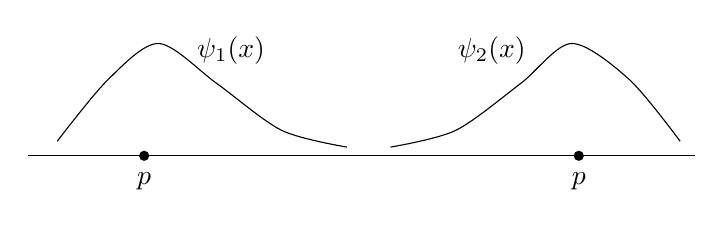
\begin{tikzpicture}[scale=0.92]
\draw (-0.2,0) -- (9.0,0);
\fill (1.4,0) circle (2pt);
\fill (7.4,0) circle (2pt);
\draw[smooth] plot coordinates {(0.2,0.2) (0.9,1.05) (1.6,1.55) (2.4,1.0) (3.3,0.35) (4.2,0.12)};
\draw[smooth] plot coordinates {(4.8,0.12) (5.7,0.35) (6.6,1.0) (7.3,1.55) (8.1,1.05) (8.8,0.2)};
\node at (1.4,-0.35) {$p$};
\node at (7.4,-0.35) {$p$};
\node at (2.6,1.45) {$\psi_1(x)$};
\node at (6.2,1.45) {$\psi_2(x)$};
\end{tikzpicture}
\caption{トンネルが許された後に平衡重ね合わせを形成するために用いられる2つの局在プロファイル。}
\lectureframe{00:17:54}
\end{figure}
\editorialnote{ラベル\(\psi_1(x)\)と\(\psi_2(x)\)は、00:17:41--00:17:56で論じられた2つのプロファイルを識別する。記号は読みやすさのために加えられた概略的ラベルである。}

無限遠の間隔では2つの状態は縮退している。電子を左に局在させるか右に局在させるかは同じエネルギーを要する。有限の間隔では新しい過程が可能になる。電子は古典的に禁じられた領域を通って一方の中心から他方へトンネルできる。障壁を通る軌道を観測しようとすれば状態を乱すであろう。``ホッピング''は量子進化の記述であり、古典的経路のフィルムではない。

平衡では電子はどちらの陽子の近くにも等しい確率で見出される。したがって規格化は因子\(1/\sqrt2\)を与え、より低い平衡状態は近似的に
\begin{equation}
\psi_+(x)\approx \frac{\psi_1(x)+\psi_2(x)}{\sqrt2}.
\end{equation}

近似記号は重要である。真の二中心波動関数は2つの無摂動水素様軌道の和では厳密にはない。それは重なり領域で調整される。ここで必要な点は、対称な平衡状態が孤立した一中心エネルギーより下にあることである。ハミルトニアンの言葉では、左と右の配置は非対角行列要素によって結合される。電子がそれらのコヒーレントな重ね合わせを占めることを許すことにより、エネルギーが下がった。

\section{低下したエネルギーから有効な力へ}

大きな陽子間隔では、電子に誘起された寄与\(E_e(r)\)は分離原子の値に近づく。より小さな間隔では、トンネルと重ね合わせがそれを下げる。完全な二陽子--一電子ポテンシャルは、陽子間の直接的反発も含まなければならない。
\begin{equation}
V_{\mathrm{tot}}(r)=V_{pp}(r)+E_e(r).
\end{equation}

これは分子の例を場のエネルギーの議論と再び結びつける。波動関数のスケッチと\(E_e(r)\)の定性的曲線は同じ計算の2つの見方であり、平衡は和\(V_{\mathrm{tot}}(r)\)によって決まる。

\begin{figure}[h]
\centering
\includegraphics[width=0.78\textwidth]{lecture_01_figure_04.png}

\medskip

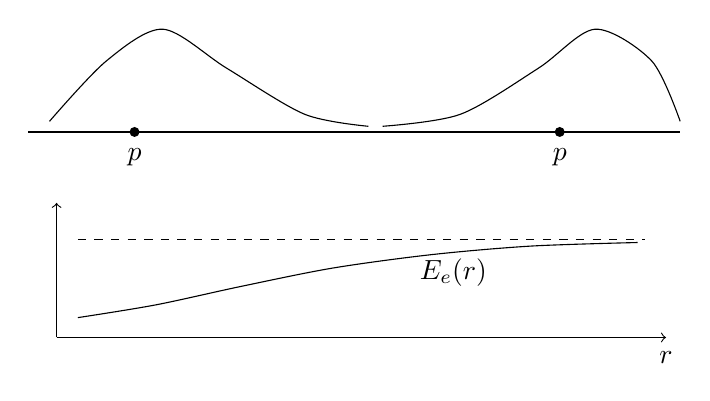
\begin{tikzpicture}[scale=0.9]
\draw (-0.2,3.0) -- (9.0,3.0);
\fill (1.3,3.0) circle (2pt);
\fill (7.3,3.0) circle (2pt);
\draw[smooth] plot coordinates {(0.1,3.15) (0.9,4.0) (1.7,4.45) (2.6,3.9) (3.7,3.25) (4.6,3.08)};
\draw[smooth] plot coordinates {(4.8,3.08) (5.9,3.25) (7.0,3.9) (7.8,4.45) (8.6,4.0) (9.0,3.15)};
\node at (1.3,2.65) {$p$};
\node at (7.3,2.65) {$p$};

\draw[->] (0.2,0.1) -- (0.2,2.0);
\draw[->] (0.2,0.1) -- (8.8,0.1);
\draw[dashed] (0.5,1.48) -- (8.5,1.48);
\draw[smooth] plot coordinates {(0.5,0.38) (1.6,0.56) (2.8,0.82) (4.1,1.08) (5.5,1.27) (6.9,1.39) (8.4,1.44)};
\node at (5.8,1.02) {$E_e(r)$};
\node at (8.8,-0.18) {$r$};
\end{tikzpicture}
\caption{上は波動関数の重なり、下は電子に誘起されたエネルギー。\(r\)が増大するにつれて分離原子の漸近値に向かって上昇する。全陽子ポテンシャルはそれらのクーロン反発も含まなければならない。}
\lectureframe{00:20:28}
\end{figure}
\editorialnote{ラベル\(E_e(r)\)と\(r\)は、00:19:12--00:20:38で論じられたエネルギー曲線と間隔を識別する。残存する板書フレームではそれらの軸ラベルは判読可能ではない。}

対応する2つの力はエネルギーの勾配から従う。
\begin{equation}
F_{e}(r)=-\frac{dE_e}{dr},
\qquad
F_{\mathrm{tot}}(r)=-\frac{dV_{\mathrm{tot}}}{dr}.
\end{equation}
したがって系はより低い全エネルギーへ押される。陽子が近づくにつれて\(E_e(r)\)が減少する場所では、交換は引力寄与を与える。束縛された間隔が存在するかどうかは、\(V_{pp}(r)\)との競合に依存する。これが共有結合の背後にある初等的機構である。電子が共有されるのは、共有状態がエネルギー的に有利だからである。

古典的計算では、電場の重なりがエネルギーを変える。ここでは、2つの力の中心がより低い量子状態を可能にする。どちらの機構も力を生むのは、平衡エネルギーが配置に依存するからである。

交換という言葉は世界線のスケッチによって要約できる。それは観測された軌道として読まれてはならない。それは電子がどちらの陽子にも結びつく振幅を表す。

\begin{figure}[h]
\centering
\begin{tikzpicture}[scale=1.0]
\draw (0,0) -- (0,4.4);
\draw (4.8,0) -- (4.8,4.4);
\draw (0,0.9) .. controls (1.6,1.7) and (3.2,1.7) .. (4.8,2.5);
\draw (4.8,2.9) .. controls (3.2,2.1) and (1.6,2.1) .. (0,3.9);
\node at (0,-0.35) {$p$};
\node at (4.8,-0.35) {$p$};
\node at (2.35,1.55) {$e^-$};
\node at (2.35,2.55) {$e^-$};
\end{tikzpicture}
\caption{2つの陽子世界線間の電子交換。観測された経路ではなく量子振幅の概略として理解される。}
\end{figure}

\begin{classroomqa}
\audiencequestion{この引力は、電子が遮蔽する、あるいは陽子の電荷を減らすという単純な描像で理解できるのか。\lecturetimestamp{00:23:26}}
\lecturerresponse{いいえ。電荷の減少はこの効果に対する正しい描像ではない。本質的な事実は、二つの局在した波動関数を加えると、それぞれの局在状態よりもわずかに低いエネルギーをもつ状態が生じるということである。}
\end{classroomqa}

\begin{classroomqa}
\audiencequestion{これが、``光は光を好む''とファインマンが言ったことの意味か。\lecturetimestamp{00:23:51}}
\lecturerresponse{いいえ。その言葉はおそらくボース統計に関するものである。光子は共通の状態を好むが、電子は排他律に従う。ここでの分子的効果は二つの中心の間のトンネル効果である。}
\end{classroomqa}

二つの陽子は依然として静電的に反発する。交換はクーロン相互作用よりも短距離的であるため、どちらか一方の寄与だけではなく全ポテンシャルを考慮しなければならない。適切な間隔では分子イオン\(\mathrm H_2^+\)はそれでも束縛される。中性の二電子系では長距離の電荷反発が存在せず、共有結合はさらに身近なものである。

\begin{classroomqa}
\audiencequestion{電子を陽子の間に置くことは、主にそれらの静電反発を減らすのか。\lecturetimestamp{00:24:33}}
\lecturerresponse{それは反発を少し減らすが、主な効果ではない。電子交換はクーロン反発よりも短距離の力である。それは中性の二電子系で最も顕著であり、そこでは原子間の長距離静電力が存在しないにもかかわらず、トンネル効果が依然として引力を生じる。}
\end{classroomqa}

\begin{classroomqa}
\audiencequestion{電子を一つしかもたない正に帯電した分子イオン\(\mathrm H_2^+\)は、実際に束縛されているのか。\lecturetimestamp{00:26:06}}
\lecturerresponse{はい。十分に小さい間隔では、交換による引力が陽子--陽子間のクーロン反発に打ち勝つのに十分な強さをもつ。}
\end{classroomqa}

\begin{classroomqa}
\audiencequestion{二中心配置は第三の力を生み出すのか。\lecturetimestamp{00:26:24}}
\lecturerresponse{新たな基本力は導入されない。二つの陽子の合成ポテンシャルにおけるSchr\"odinger方程式は、一中心問題とは異なる平衡エネルギーをもち、その変化したエネルギーの導関数が有効力である。}
\end{classroomqa}

\begin{classroomqa}
\audiencequestion{このエネルギーの低下は量子もつれの例か。\lecturetimestamp{00:27:06}}
\lecturerresponse{通常の二粒子の意味ではない。必要な電子は一つだけである。関連する数学的特徴は、左と右の状態を結合する非対角ハミルトニアン行列要素である。}
\end{classroomqa}

\begin{classroomqa}
\audiencequestion{高温では交換はどうなるのか。\lecturetimestamp{00:27:37}}
\lecturerresponse{極端な温度では電子は電離し、分子のことをまったく忘れてしまう。より低い励起エネルギーでは、電子はより大きな軌道を占めることがあり、重なりが変化し、したがって力も変化する。これは状態に依存する補正であり、新たな一般的機構ではない。}
\end{classroomqa}

\section{光子交換と表の最初の項目}

クーロン力を同じ交換の言葉で説明できるだろうか。荷電粒子は電磁場と相互作用し、その量子は光子である。古典的には電荷の周りの電場を解く。量子場の理論では、その相互作用を光子の放出と吸収に分解する。

物理的な荷電粒子は単なる裸の電荷ではない。その状態は、裸の電子成分、光子を一つもつ電子、光子を二つもつ電子などを含む量子重ね合わせである。意図的に模式的な記法で書けば、
\begin{equation}
\begin{aligned}
\ket{e_{\mathrm{phys}}}
={}&a_0\ket e
+a_1\ket{e+\text{one photon}}
\\
&+a_2\ket{e+\text{two photons}}+\cdots .
\end{aligned}
\end{equation}
この記法は光子数の成分の階層のみを記録しており、光子の運動量を指定したり、相互作用する荷電状態の完全な構成を試みたりするものではない。
周囲の光子は自由な放射として逃げるのではなく、放出され再吸収される。その効果は測定できるが、自由に伝播する光子と同じ方法で検出されるわけではない。第二の電荷を近くに置くと、一方の電荷で放出された光子が他方で吸収されうる。そのとき二つのドレスされた状態は、二つの孤立したエネルギーの単純な和に等しいエネルギーをもたなくなる。

教室での類推は、それぞれが一組のボールを扱う二人のジャグラーである。彼らが遠く離れているときは、それぞれが独立にジャグリングする。十分に近づけると、一方が他方の投げたボールを捕まえるかもしれない。ファインマン図の言葉では、その共有された対象が交換される光子である。この類推は微視的な軌道ではないが、近接がなぜ新たな過程を可能にするかを捉えている。

今や、クーロンの法則を単に暗記することを超えた二つの記述が手に入った。古典場の理論は場を加え、その結果を二乗する。量子場の理論は、量子が交換される振幅を足し合わせる。この意味で、粒子、場、力は一対一対一の対応をなしている。電子は分子の交換を媒介し、光子は電磁的な交換を媒介し、交換されうる任意の粒子は適切な設定において力に寄与しうる。したがって、自然界には四つの基本的相互作用があるというよく知られた言明は、より広い階層での分類である。交換の言語の内部では、交換可能な種それぞれが独自の有効な力の寄与を生み出しうる。

いよいよ、粒子に名前を付け、その性質を列挙し、どの過程に入りうるかを述べる時である。標準模型の全体を一度に書き下すことは、長い記憶力テストを生むだけなので、粒子を、その構成要素が単純に関連し合う小さな群に分け、各群が何をなしうるかを学ぶことにしよう。

完全な目録が厄介なのは、なぜまさにこれらの粒子が存在し、他の想像しうる粒子は存在しないのかを、我々が理解していないからである。数学的な整合性はいくつかの関係を与える。すなわち、あるパターンのいくつかの構成要素が存在すれば、それを完成させるために別の構成要素が要求されうる。それらの関係は独立な事実の数を減らすが、その減り方はわずかな倍率にとどまる。多くの粒子の種類と多くのパラメータが未解明のまま残る。その未完成な構造を理解することは、後の実験が何を発見しようとしているのかを理解するために必要である。

\begin{figure}[h]
\centering
\includegraphics[width=0.7\textwidth]{lecture_01_figure_05.png}
\caption{粒子表の最初の項目は、光子を\(\gamma\)によって、その場をベクトルポテンシャル\(A\)によって同定する。}
\lectureframe{00:39:11}
\end{figure}

最初の場--量子の同定は
\begin{equation}
\gamma \leftrightarrow A.
\end{equation}
ここで\(A\)は電磁ベクトルポテンシャルである。光子はスピン1のボソンであり、電荷ゼロ、バリオン数ゼロ、静止質量ゼロをもつ。電子場は慣例的に\(\psi_e\)と表記され、その生成と消滅の部分は電子状態と陽電子状態に作用する。

我々の表は、名前、粒子記号、場、ボソンかフェルミオンかの型、電荷\(Q\)、バリオン数\(B\)、質量を記録する：

\begin{table}[h]
\centering
\resizebox{\linewidth}{!}{%
\begin{tabular}{lllllll}
名前&記号&場&型&\(Q\)&\(B\)&質量\\
光子&\(\gamma\)&\(A\)&ボソン&\(0\)&\(0\)&\(0\)\\
電子&\(e^-\)&\(\psi_e\)&フェルミオン&\(-1\)&\(0\)&\(0.51\,\mathrm{MeV}\)\\
陽電子&\(e^+\)&\(\psi_e\)&フェルミオン&\(+1\)&\(0\)&\(0.51\,\mathrm{MeV}\)
\end{tabular}
}%
\caption{粒子目録を始める光子と電子--陽電子の項目。}
\end{table}

電子と陽電子の関係は相互的である。すなわち、それぞれが他方の反粒子である。負に帯電した状態``を粒子''と呼ぶのは慣例である。我々は電荷を電子電荷の大きさの単位で測るので、
\begin{equation}
Q(e^-)=-1,\qquad Q(e^+)=+1.
\end{equation}
質量は\(E=mc^2\)を用いてエネルギー単位で測られる。1電子ボルトは、電荷\(e\)が1ボルトの電位差を通って得るエネルギーである：
\begin{equation}
1\,\mathrm{eV}=e\,(1\,\mathrm V).
\end{equation}
この単位は原子物理学から自然に生じる。粗い原子スケールとして、水素を電離するにはおよそ\(13.5\,\mathrm{eV}\)かかる。粒子の質量には数百万または数十億電子ボルトが必要である。電子の質量は
\begin{equation}
m_e c^2 \approx 0.511\,\mathrm{MeV}.
\end{equation}

\begin{classroomqa}
\audiencequestion{電子の質量は正確にMeVの半分であるべきか？\lecturetimestamp{00:44:02}}
\lecturerresponse{いいえ。都合のよい丸めた値\(0.51\,\mathrm{MeV}\)は、いかなる原理によっても正確に半分に固定されているわけではなく、測定されたパラメータである。}
\end{classroomqa}

素朴なQED過程は、1本の荷電フェルミオン線が入り、1本が出て、1本の光子線が付着している。脚を並べ替えたり交差させたりすることで、同じ頂点が光子の放出、吸収、または陽電子の過程を記述できる。ここで用いる非共変的な図式的記法では、相互作用は次を含む：
\begin{equation}
\mathcal{L}_{\mathrm{int}}\sim e\,\psi_e^\dagger \psi_e A.
\end{equation}
場を生成演算子と消滅演算子に展開すると、入射電子を消し、出射電子を生成し、光子を生成または消滅させる項が生じる。結合\(e\)は頂点で1つの因子を与える。したがって、電子が散乱または加速される際の光子放出に対して、
\begin{equation}
\mathcal{A}_{\mathrm{vertex}}\propto e,
\qquad
P_{\mathrm{emission}}\propto e^2.
\end{equation}
X線管で電子が標的に当たることは、この光子放出確率が重要となる実用的な設定の一つである。同じ頂点の繰り返しの組み合わせが、電荷間の力として解釈されるエネルギーシフトを含む量子電磁力学の過程を生み出す。

したがって、模式的な頂点が有用である。

\begin{figure}[h]
\centering
\begin{tikzpicture}[scale=1.0]
\fill (0,0) circle (1.5pt);
\draw (-1.6,-1.2) -- (0,0) -- (1.6,-1.2);
\draw (0,0) -- (0,1.8);
\node at (-1.8,-1.4) {$e^-$};
\node at (1.8,-1.4) {$e^-$};
\node at (0.35,1.95) {$\gamma$};
\end{tikzpicture}
\caption{素電磁相互作用の基本頂点の位相的模式図：荷電フェルミオン線が1本入り、1本出て、光子が1本付着している。ここで直線的な光子の脚は単なる簡略化された作図上の約束である。}
\end{figure}

力への交換寄与は、そのような頂点を2つ結び合わせる：

\begin{figure}[h]
\centering
\begin{tikzpicture}[scale=1.0]
\draw (0,0) -- (0,4.0);
\draw (4.8,0) -- (4.8,4.0);
\draw (0,2.0) -- (4.8,2.0);
\node at (0,-0.35) {$e^-$};
\node at (4.8,-0.35) {$e^-$};
\node at (2.4,2.3) {$\gamma$};
\end{tikzpicture}
\caption{光子交換の位相的模式図であり、クーロン相互作用の量子場理論的記述を与える。}
\end{figure}

粒子--場--力の三角形が閉じたので、目録を続けることができる。

\section{クォーク、バリオン数、そして世代の謎}

この目録が1960年頃に書かれていたなら、陽子と中性子はおそらく電子と光子に続いていたであろう。現代の素粒子物理学はクォークを先に挿入する。素朴な構成子描像では、陽子と中性子はより小さなクォーク自由度からなる比較的大きな複合体である。\emph{複合体}の正確な意味はまだ検討されるべきであるが、構成子という言葉はすでに極めて有用である。

すべてのクォークはフェルミオンである。それらは核物理学において核子を数えることによって導入された量であるバリオン数を担う。\emph{核子}とは具体的に陽子または中性子を意味する。\emph{バリオン}は核子および後に出会う同様の重い粒子を含む、より広いクラスである。陽子と中性子はそれぞれ1単位を持ち、
\begin{equation}
B(p)=B(n)=1,
\qquad
B(\bar p)=B(\bar n)=-1.
\end{equation}
原子核に対して、このバリオン数はちょうど質量数\(A=Z+N\)、すなわち陽子数と中性子数の和である。原子質量単位で測った数値的な原子質量は\(A\)にほぼ等しいだけである。ベータ過程では陽子が中性子に、中性子が陽子に変わりうるが、核子の総数は変わらない。例えば、
\begin{equation}
n\longrightarrow p+e^-+\bar\nu_e
\end{equation}
は陽子数と中性子数を別々に変えるが、その和は保つ。

\begin{classroomqa}
\audiencequestion{同位体は陽子数と中性子数の和の保存に反するか？\lecturetimestamp{00:52:03}}
\lecturerresponse{異なる同位体は確かに異なる中性子数を含み、ベータ崩壊は中性子と陽子を入れ替えうる。通常の核過程で関係する保存量は、どちらかの種別ではなく全バリオン数である。}
\end{classroomqa}

規格化は慣習的である。陽子にバリオン数\(2\)、\(7\)、または\(\pi\)を割り当てても、すべての複合体が整合的にスケールされる限り問題ない。陽子に\(B=1\)を割り当て、それが3つのクォークを含むなら、各クォークは
\begin{equation}
B(q)=\frac13,
\qquad
B(\bar q)=-\frac13.
\end{equation}
を持たねばならない。したがって分数値は、複合体である核子を先に規格化したことの歴史的帰結である。

\begin{classroomqa}
\audiencequestion{クォークの数は保存されるか？\lecturetimestamp{00:54:23}}
\lecturerresponse{クォーク--反クォーク対は生成・消滅しうるので、生の数は保存されない。バリオン数に対応する量は、クォーク数から反クォーク数を引いて3で割ったものである。経験的には極めて高い精度で保存されているが、ここでは絶対的な法則であるとは仮定されていない。}
\end{classroomqa}

例えば
\begin{equation}
p\longrightarrow e^++\gamma
\end{equation}
のような仮想的な電荷保存崩壊は、バリオン数1をバリオン数0の終状態へ持ち込むであろう。このチャネルは例示的な帳簿上の例であり、提案された崩壊模型ではない。バリオン数を破る過程は観測されていない。ここで引用された粗い上限は、陽子の寿命を少なくとも\(10^{33}\)--\(10^{34}\)年の範囲に置く。その長さの間、単一の陽子を観測するのではない。膨大な数の陽子を扱いやすい時間だけ観測し、寿命と試料サイズを交換するのである。それにもかかわらず陽子崩壊は広く期待されており、ここで議論されている数学の何も絶対的な禁止を与えなかった。したがってバリオン数が厳密であるかどうかは、未解決の実験的問題であり続けた：未観測で、強く制約されているが、否定されてはいない。

\begin{classroomqa}
\audiencequestion{陽子--反陽子対消滅はバリオン数に反するか？\lecturetimestamp{00:56:17}}
\lecturerresponse{反しない。初期のバリオン数は\(1+(-1)=0\)なので、バリオン数0の終状態への対消滅はそれを保存する。非バリオン的生成物へ崩壊する孤立した陽子こそが破れであろう。}
\end{classroomqa}

クォークには6つのフレーバーがあり、
\begin{equation}
u,\ d,\ s,\ c,\ b,\ t,
\end{equation}
アップ、ダウン、ストレンジ、チャーム、ボトム、トップと呼ばれる。アップクォークに上向きなところは何もなく、ストレンジクォークは隣人より奇妙でもない。名前は論理ではなく歴史を記録している。場の記法は完全には一様でない：場とその量子の両方に対して\(q\)、\(Q\)、\(\psi_q\)、あるいは単にフレーバー文字\(u,d,s,c,b,t\)に出会う。

\begin{classroomqa}
\audiencequestion{ボトムとトップは、かつてビューティーとトゥルースと呼ばれていたのと同じ粒子ですか。\lecturetimestamp{00:58:35}}
\lecturerresponse{はい。より飾り気の少ない名前であるボトムとトップが標準となった。この命名の歴史には力学的な内容はない。}
\end{classroomqa}

それらの電荷は三つの対で繰り返される：
\begin{equation}
\begin{aligned}
Q(u)=Q(c)=Q(t)&=+\frac23,
\\
Q(d)=Q(s)=Q(b)&=-\frac13.
\end{aligned}
\end{equation}
反クォークは反対の電荷とバリオン数を持つ。孤立した分数電荷は決して見られない。なぜならクォークは自由な漸近粒子として存在せず、観測されるハドロンは整数の電荷を持つからである。

対 \((d,u)\)、\((s,c)\)、\((b,t)\) は同じ電荷パターンを繰り返す三つの世代である。六つすべてが依然として \(B=1/3\) を持つ。

\begin{classroomqa}
\audiencequestion{より重いクォークもバリオン数 \(1/3\) を持つのですか。\lecturetimestamp{01:02:02}}
\lecturerresponse{はい。すべてのクォークはバリオン数 \(1/3\) を持つ。}
\end{classroomqa}

質量には比較できるほどの繰り返しは見られない。有用な桁程度の値は
\begin{align}
m_u &\sim 5\,\mathrm{MeV},
&
m_d &\sim 10\,\mathrm{MeV},
\\
m_s &\sim 100\,\mathrm{MeV},
&
m_c &\sim 10^3\,\mathrm{MeV},
\\
m_b &\sim 5\,\mathrm{GeV},
&
m_t &\sim 170\,\mathrm{GeV}.
\end{align}
ここで \(1\,\mathrm{GeV}=10^3\,\mathrm{MeV}\) である。単位の変更により、ボトムクォークとトップクォークの項目は読みやすく保たれる。ダウンクォークの推定値は電子の \(0.511\,\mathrm{MeV}\) よりはるかに大きいが、陽子のおおよそ \(940\,\mathrm{MeV}\) よりはるかに小さく、約 \(1{,}800\) 電子質量である。実際、二つの軽いアップクォークの項目と一つのダウンクォークの項目を加えても陽子の質量には近づかない。ハドロンのエネルギーの残りは最終的に説明されなければならない。

\editorialnote{口頭の比較では \(10\,\mathrm{MeV}\) のダウンクォークを約五十電子質量と呼んだ。ここに書かれた粗い値を用いると \(10/0.511\approx20\) である。階層は正しいが、五十という因子は算術的なミスである。}

対の中での順序さえも繰り返されない。ダウンクォークはアップより重いが、チャームはストレンジよりはるかに重い。トップはアップクォークの数万倍重いが、それらの電荷と相互作用のパターンは密接に類似している。

ここには実際に二つの謎がある。なぜ一つのクォーク世代さえ存在するのかを我々は理解していない。ただし第一世代は少なくとも陽子、中性子、通常の物質に必要なアップクォークとダウンクォークを供給する。また、なぜ自然がそのパターンを第二世代と第三世代で繰り返すのか、あるいはなぜ繰り返された粒子の質量がこれほど多くの桁にわたって散らばっているのかも理解していない。アイデアはあるが、このパターンを計算する受け入れられた説明はない。

\begin{classroomqa}
\audiencequestion{トップクォークの質量に根本的な説明がないのなら、直接発見の前にそのおおよその値はどのように予想されたのですか。\lecturetimestamp{01:05:53}}
\lecturerresponse{その推定はより深い原理から質量を導いたものではない。候補の質量を仮定し、仮想トップクォークがよく測定された過程に影響するダイアグラムを計算し、どの値がそれらの観測と整合するかを問うのである。間接的な感度は、自然がなぜそれを選んだかを説明することなく、パラメータを特定できる。}
\end{classroomqa}

\begin{classroomqa}
\audiencequestion{自由なクォークを孤立させられないのなら、どのような意味でクォークを検出できるのですか。\lecturetimestamp{01:08:04}}
\lecturerresponse{クォークの証拠は検出可能である。それらの生成は特徴的なエネルギー、方向、粒子ジェットを残し、仮想クォークは他の観測量に影響する。準備できないのは、すべてのハドロンの相棒から分離され、孤立した漸近粒子として調べられる単独のクォークである。}
\end{classroomqa}

\begin{classroomqa}
\audiencequestion{電荷 \(-1/3\) と \(+2/3\) のパターンは理論から導かれるのですか、それとも単なる帳簿付けですか。\lecturetimestamp{01:09:02}}
\lecturerresponse{パターンの一部は数学的整合性によって要求されるが、一部にすぎない。この段階では電荷は事実として記録されている。整合性の条件は、標準模型のより多くが整った後に初めて議論される。}
\end{classroomqa}

通常の物質中で相当な存在量を持つのは \(u\) と \(d\) クォークだけである。より重いフレーバーはより軽い状態へ崩壊する。したがってアップクォークとダウンクォークの相対存在量は、主に陽子と中性子の宇宙的および核的な存在量と、それらの構成内容によって決まる。

\begin{classroomqa}
\audiencequestion{宇宙における六つのクォークフレーバーの相対存在量を決めるものは何ですか。\lecturetimestamp{01:09:49}}
\lecturerresponse{安定な物質は本質的にアップクォークとダウンクォークを含み、より重いフレーバーは崩壊する。自由中性子は崩壊するが、陽子は観測される時間スケールでは安定である。ただし中性子は原子核に束縛されているときは豊富に残る。するとアップクォークとダウンクォークの数え上げは、この段階ではそれらの陽子と中性子の数え上げに帰着する。}
\end{classroomqa}

\section{クォークからハドロンへ：核子、ストレンジバリオン、中間子}

クォークの電荷が分かれば、おなじみのハドロンを再構成できる。中性子と陽子はそれぞれ三つの価クォークを含む：
\begin{equation}
n=ddu,
\qquad
p=uud.
\end{equation}
それらの電荷は直ちに確認できる：
\begin{align}
Q(n) &= Q(d)+Q(d)+Q(u)
= -\frac13-\frac13+\frac23
=0,\\
Q(p) &= Q(u)+Q(u)+Q(d)
= \frac23+\frac23-\frac13
=1.
\end{align}

しばらく光子のことは忘れよう。電磁気学を切り離すと、陽子と中性子は、\(u\) と \(d\) を入れ替えただけのほとんど同じ対象のように見える。この近似的対称性は厳密ではない。2つのクォークの質量が厳密に等しいわけではないからである。対応する軽い中間子に出会った後で初めて、この対称性に名前を与え、展開する。

\(m_d>m_u\) であるから、2つのダウンクォークを含む中性子の方が、クォーク質量からの寄与をより大きく受けるはずである。電磁的自己エネルギーは逆方向に働く。荷電した陽子は電場のエネルギーを蓄えるが、中性子は正味の電荷を持たない。自然はこの競合を、わずかに重い中性子という形で解決している。この粗い近似の水準では、
\begin{align}
m_pc^2&\approx940\,\mathrm{MeV},\\
m_nc^2&\approx940\,\mathrm{MeV},\\
(m_n-m_p)c^2&\approx1.4\,\mathrm{MeV}.
\end{align}

\begin{classroomqa}
\audiencequestion{陽子と中性子の質量はいくらか。\lecturetimestamp{01:15:35}}
\lecturerresponse{どちらも \(940\,\mathrm{MeV}\) 付近にあり、この粗い水準では差は約 \(1.4\,\mathrm{MeV}\) である。}
\end{classroomqa}

それでも、この小さな超過分は自由中性子の崩壊を可能にするのに十分である。電子の静止エネルギーを支払った後、残りのエネルギーは \(n\to p+e^-+\bar\nu_e\) における運動エネルギーとして現れうる。

同じ構成要素の論理からストレンジバリオンが生じる。\(s\) と \(d\) は同じ電荷を持つので、電荷のパターンを変えずにダウンクォークをストレンジクォークに置き換えられる。
\begin{equation}
uds,\qquad uss,\qquad uus.
\end{equation}
したがって、上の例では \(uds\) と \(uss\) は中性であり、\(uus\) は電荷 \(+1\) を持つ。このような状態には \(\Lambda\) や \(\Xi\) を含む名前が与えられた。この段階では、それらの名前の詳細な割り当ては必要ない。\(d\) を \(s\) に置き換えることは、関連する原子核で一方の核子種をもう一方に置き換えることと定性的に類似している。結合のパターンの多くは保たれるが、構成要素の変化が質量をずらす。これらの状態は通常の核子より重く、エネルギーと他の保存量子数を運ぶために必要な追加の粒子とともに、より軽いバリオンへ崩壊する。

\begin{classroomqa}
\audiencequestion{ストレンジバリオンが崩壊すると何が現れるか。\lecturetimestamp{01:19:02}}
\lecturerresponse{陽子や中性子のようなより軽いバリオンが現れるが、それが唯一の生成物ではありえない。余分なエネルギーと保存量子数のために追加の粒子が必要である。詳細な崩壊規則は後回しにする。}
\end{classroomqa}

詳細な置換規則はこの最初の目録より複雑であるが、安全な操作の1つは、あるフレーバーを同じ電荷を持つ別のフレーバーに置き換えることである。ダウンクォークをストレンジクォークに置き換えると、この粗い構成要素の水準ではおよそ \(90\,\mathrm{MeV}\) が加わる。したがってこれらのバリオンは陽子や中性子よりいくらか重い。より軽い核子へ崩壊しうるため、通常の物質中や我々の周囲の宇宙には豊富には存在しない。

\begin{classroomqa}
\audiencequestion{すべてのバリオンには、各クォークをその反クォークに置き換えて作られる反バリオンがあるか。\lecturetimestamp{01:20:33}}
\lecturerresponse{はい。すべての構成要素をその反粒子に置き換えると、反陽子、反中性子、または対応する反ストレンジバリオンが生成され、すべての加法的電荷が反転する。}
\end{classroomqa}

\begin{classroomqa}
\audiencequestion{ストレンジクォークの代わりにボトムクォークに置き換えるとどうなるか。\lecturetimestamp{01:21:00}}
\lecturerresponse{結果はボトムバリオンである。``ストレンジバリオン'' とは、特に \(s\) クォークが存在することを意味する。この形容詞はフレーバーを名指ししており、一般的な不慣れさの度合いを表すものではない。}
\end{classroomqa}

\emph{ストレンジ} という形容詞は、物理学者が陽子と中性子に親しみ、新たに発見された粒子がそれらの隣で予想外に見えた後に生じた。フレーバー構造が分かれば、それらの存在は他のどのクォーク複合体よりも奇妙なものではない。

構成要素の質量は重要な警告を露呈する。2つのアップクォーク質量と1つのダウンクォーク質量を足しても数十 MeV にしかならず、陽子のおよそ \(940\,\mathrm{MeV}\) にはまったく及ばない。その素朴な和には何か実質的なものが欠けている。陽子と中性子はグルーオンも含み、グルーオンはエネルギーを運ぶ。相対論的束縛系では、複合体の質量は構成要素の列挙された質量を単純に足すだけでは得られない。

\begin{classroomqa}
\audiencequestion{見かけ上欠けている陽子と中性子の質量はどこから来るのか。グルーオンは質量を運ぶのか。\lecturetimestamp{01:21:26}}
\lecturerresponse{この帳簿付けではグルーオンはバリオン数を運ばないが、エネルギーは運ぶ。そのエネルギーは、陽子や中性子の質量が軽いクォークの質量の項目の和にならない理由の一部である。}
\end{classroomqa}

\begin{classroomqa}
\audiencequestion{その欠けている寄与は結合エネルギーの一種か。\lecturetimestamp{01:22:03}}
\lecturerresponse{はい、結合エネルギーの一種と呼んでよい。警告は、相対論的複合体の質量は、構成要素の質量パラメータを足すことで示唆される単純な足し算には従わないということである。}
\end{classroomqa}

\begin{classroomqa}
\audiencequestion{複合的な陽子は、粒子の言葉だけでなく場の言葉でも記述できるのでしょうか。\lecturetimestamp{01:22:45}}
\lecturerresponse{はい、できますが、はるかに困難です。ここで展開している構成要素の帳簿付けには、空間的に広がった場を直接組み合わせようとするよりも、粒子の言葉の方がはるかに透明です。}
\end{classroomqa}

\begin{classroomqa}
\audiencequestion{通常の結合エネルギーは、分離した構成要素に対して負です。なぜ核子の動的寄与は大きな正のエネルギーなのでしょうか。\lecturetimestamp{01:23:32}}
\lecturerresponse{通常の負の結合という直感は、この場合には当てはまりません。説明は強い相互作用の後半の扱いに属するので、今はこの問いは保留されます。}
\end{classroomqa}

なぜ3つのクォークはバリオンを形成するのに、2つのクォークは孤立した2クォークハドロンを形成しないのでしょうか。クォーク理論の初期には、これは真の難問でした。観測される束縛された組み合わせは、電気素量の整数倍に等しい電荷を持たなければならない、と答えることもできるでしょう。それだけでは循環論のように聞こえます。それは説明せずにパターンを記述しているからです。それでも、この規則は正しい方向を指していることが判明し、そのより深い起源は、強い相互作用のより多くが整って初めて理解できます。今のところ、これは明示的に作業規則です。3つのクォークはバリオンを作ることができ、クォークと反クォークは中間子を作ることができ、その結果観測される複合体は整数の電荷を持ちます。

3つの同一の軽いフレーバーから作られるバリオンも存在しますが、その詳細は中間子の後まで待つことができます。

中間子は\(q\bar q\)複合体です。そのバリオン数は消えます。
\begin{equation}
B(q\bar q)=\frac13-\frac13=0.
\end{equation}
最も軽い例は\(u\)と\(d\)を使います。これらのフレーバーは他のものよりずっと軽く、通常の物質中で安定であるか比較的ゆっくりと消え、自然界に豊富に存在します。それらの低い生成閾値はまた、衝突が重いフレーバーよりもそれらを容易に作ることを意味します。これらすべての理由から、軽いクォークの複合体は実験的に最初に出会う中間子であり、始めるのに自然な場所です。

自然なフレーバー基底は
\begin{equation}
\ket{\bar u d},\qquad \ket{u\bar d},\qquad \ket{\bar u u},\qquad \ket{\bar d d}.
\end{equation}
この最初の数え上げでは追加の制限は使われません。4つの軽いクォーク--反クォークの対形成はすべて保持され、それらの電荷が計算されます。

荷電状態はすぐに得られます。\(Q(\bar u)=-2/3\)と\(Q(d)=-1/3\)なので、
\begin{align}
Q(\bar u d)&=-\frac23-\frac13=-1,
&
\ket{\pi^-}&=\ket{\bar u d}.
\end{align}
すべての構成要素を反粒子に置き換えると\(u\bar d\)が得られるので、2番目の状態は最初の状態の反粒子です。
\begin{align}
Q(u\bar d)&=+\frac23+\frac13=+1,
&
\ket{\pi^+}&=\ket{u\bar d}.
\end{align}

同一フレーバーの状態は中性ですが、どちらも単独では別の粒子名を持ちません。量子力学はそれらを重ね合わせることを許します。2つの規格化された直交する組み合わせは
\begin{align}
\ket{\pi^0} &\approx \frac{\ket{\bar u u}-\ket{\bar d d}}{\sqrt2},\\
\ket{\eta} &\approx \frac{\ket{\bar u u}+\ket{\bar d d}}{\sqrt2}.
\end{align}

\begin{figure}[h]
\centering
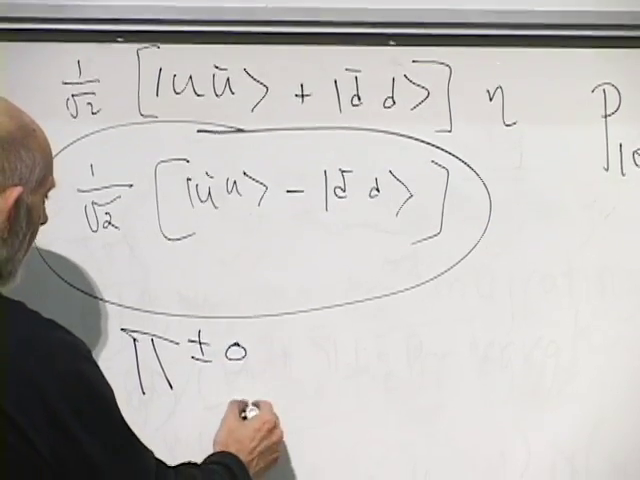
\includegraphics[width=0.82\textwidth]{lecture_01_figure_06.png}
\caption{対称な中性の組み合わせは\(\eta\)と同定され、反対称な組み合わせはパイ中間子三重項にまとめられます。}
\lectureframe{01:32:35}
\end{figure}

各中性状態は、通常のスピンではなく、\emph{アップネス}と\emph{ダウンネス}を通じてもつれたクォーク--反クォーク対です。アップとダウンのフレーバーがスピン1/2変数の2つの方向のように数学的に扱われるなら、上の和と差はおなじみの2スピン重ね合わせと同じ役割を果たします。このスピンの内部類似物は\emph{アイソスピン}と呼ばれます。空間内で文字通り上や下を指しているものは何もありません。2つの方向は\(u\)と\(d\)のフレーバーをラベル付けします。

3つのパイ中間子\(\pi^+\)、\(\pi^0\)、\(\pi^-\)はアイソスピン三重項を形成します。それらの質量はほぼ等しく、アップクォークとダウンクォークが正確に同じ質量を持てば、より近く一致するでしょう。直交する中性状態は\(\eta\)と呼ばれます。

\(\eta\)はパイ中間子よりかなり重いです。
\begin{equation}
m_\pi \approx 140\,\mathrm{MeV},
\qquad
m_\eta \approx 500\,\mathrm{MeV}.
\end{equation}
なぜ\(\eta\)が際立つのかは長い間不明でした。説明は今では理解されていますが、数学的に抽象的であり、ここでは展開されません。

\begin{classroomqa}
\audiencequestion{これらの中間子は比較的長寿命なのでしょうか。\lecturetimestamp{01:33:59}}
\lecturerresponse{多くの強く崩壊する粒子に比べて、はい。それらは議論中のチャネルで強い相互作用を通じて崩壊しません。弱い崩壊と電磁崩壊がそれらをより長寿命にします。}
\end{classroomqa}

\begin{classroomqa}
\audiencequestion{個々の中性状態\(\bar u u\)と\(\bar d d\)は独自の名前を持っていますか。\lecturetimestamp{01:34:29}}
\lecturerresponse{いいえ。名前を持つ粒子は、それらの和と差によって形成される線形結合です。それらの組み合わせは確定した値を持ちます。}
\end{classroomqa}

\begin{classroomqa}
\audiencequestion{この中性状態の重ね合わせはニュートリノ振動のようなものですか。\lecturetimestamp{01:34:44}}
\lecturerresponse{両者が量子重ね合わせを含むという限られた意味では似ている。ここでの問題は、2つのスピン1/2の構成要素からなるスピンの組み合わせと、そのような状態がもつれ合う2つの仕方により密接に関係している。その議論は次回の講義に譲る。}
\end{classroomqa}

ストレンジクォークを導入すると、\(d\)または\(\bar d\)を\(s\)または\(\bar s\)で置き換えることにより、4つのストレンジまたは\(K\)中間子のフレーバー状態が得られる。
\begin{equation}
\bar u s,\qquad u\bar s,\qquad \bar d s,\qquad d\bar s.
\end{equation}
それらの電荷の割り当ては
\begin{align}
Q(\bar u s) &=-1,
&
Q(u\bar s) &=+1,
\\
Q(\bar d s) &=0,
&
Q(d\bar s) &=0.
\end{align}
したがって、2つの荷電K中間子と2つの中性K中間子が存在する。

最初の数え上げでは、3つのパイ中間子、4つのK中間子、そして1つの\(\eta\)が得られる。すなわち8つの状態である。しかし、このリストはまだ\(\ket{s\bar s}\)の対を用いていない。3つのフレーバーと3つの反フレーバーがあるので、完全な基本的な数え上げはしたがって
\begin{equation}
3\times3=9.
\end{equation}
となる。欠けていた\(s\bar s\)状態が、9つのクォーク--反クォークフレーバー組み合わせの数え上げを完成させる。
